\FloatBarrier
\begin{figure}[h]
\centering
%\begin{minipage}{0.65\textwidth}
\resizebox{\columnwidth}{!}{
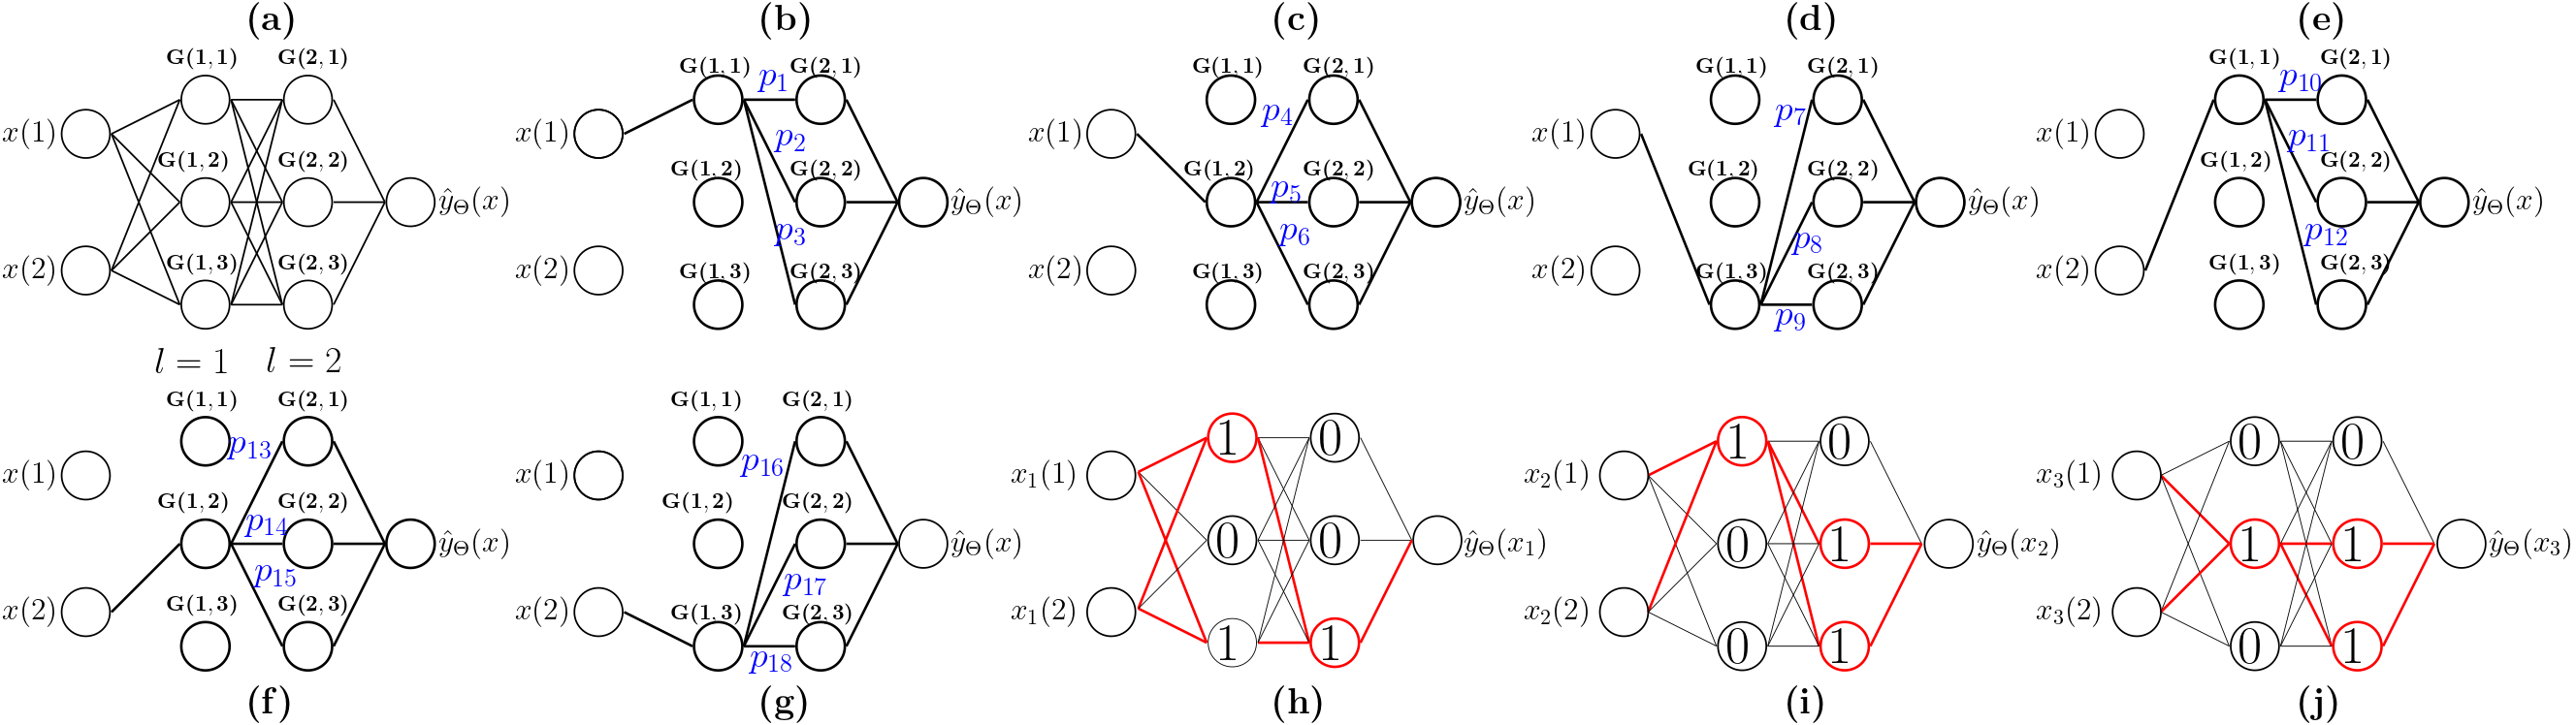
\includegraphics[scale=1]{figs/npf-npk-flipped.png}
}
\centering
%\resizebox{\columnwidth}{!}{
%$\phi_{x}=[x(1)A(x,p_1),\ldots,x(1)A(x,p_{9}),x(2)A(x,p_{10}),\ldots,x(2)A(x,p_{18})]^\top, \phi_{x_1}=[0, 0, x_1(1),0,0, 0, 0,0, x_1(1), 0, 0, x_1(2),0, 0, 0,0, 0, x_1(2)]^\top$
%}
%\resizebox{\columnwidth}{!}{
%$\phi_{x_2}=[0, x_2(1), x_2(1),0,0, 0, 0,0,0, 0, x_2(2), x_2(2),0,0, 0, 0,0,0 ]^\top, \phi_{x_3}=[0, 0,0,0, x_3(1),x_3(1),0,0, 0,0, 0,0,0, x_3(2),x_3(2),0,0, 0 ]^\top$
%}
\begin{minipage}{0.64\textwidth}
%\resizebox{\columnwidth}{!}{
%$\phi_{x}=[x(1)A(x,p_1),\ldots,x(1)A(x,p_{9}),x(2)A(x,p_{10}),\ldots,x(2)A(x,p_{18})]^\top$
%}
%\\
\resizebox{\columnwidth}{!}{
$\phi_{x_1}=[0, 0, x_1(1),0,0, 0, 0,0, x_1(1), 0, 0, x_1(2),0, 0, 0,0, 0, x_1(2)]^\top$
}
\\
\resizebox{\columnwidth}{!}{
$\phi_{x_2}=[0, x_2(1), x_2(1),0,0, 0, 0,0,0, 0, x_2(2), x_2(2),0,0, 0, 0,0,0 ]^\top$
}
\\
\resizebox{\columnwidth}{!}{
$\phi_{x_3}=[0, 0,0,0, x_3(1),x_3(1),0,0, 0,0, 0,0,0, x_3(2),x_3(2),0,0, 0 ]^\top$
}
\end{minipage}
\begin{minipage}{0.25\textwidth}
%\resizebox{\columnwidth}{!}{
,\,$\Lambda=\left[\begin{matrix} 
2 &1& 0 \\
1 &2& 0\\
0 &0& 2
\end{matrix}\right]$
%}
\end{minipage}

\begin{comment}
\begin{minipage}{0.4\textwidth}
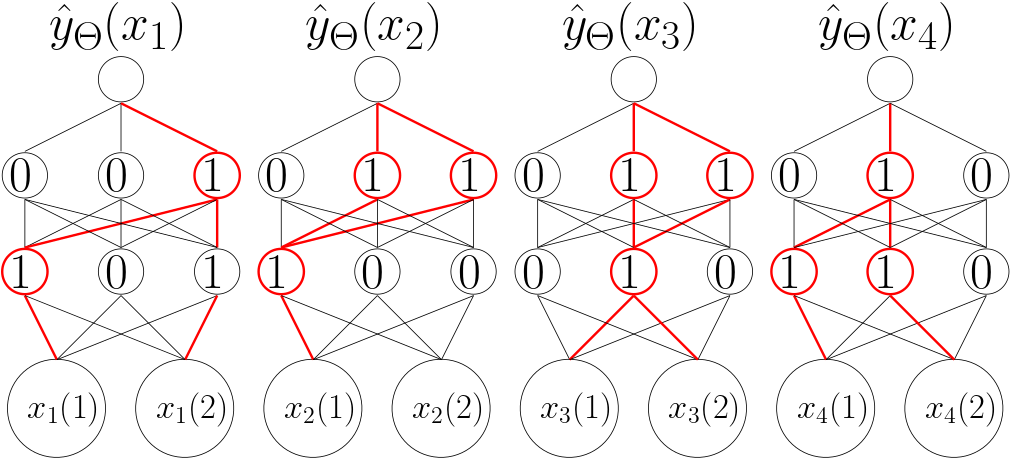
\includegraphics[scale=0.15]{figs/npf-npk.png}
\end{minipage}
\begin{minipage}{0.55\textwidth}
%\resizebox{\columnwidth}{!}{
%$\phi_{x,\Theta}=[x(1)A_{\Theta}(x,p_1),\ldots, x(1)A_{\Theta}(x,p_9),x(2)A_{\Theta}(x,p_{10}),\ldots, x(2)A_{\Theta}(x,p_{18})]^\top$
%}
%\\
\resizebox{\columnwidth}{!}{
$\phi_{x_1,\Theta}=[0, 0, x_1(1),0,0, 0, 0,0, x_1(1), 0, 0, x_1(2),0, 0, 0,0, 0, x_1(2)]^\top$
}
\\
\resizebox{\columnwidth}{!}{
$\phi_{x_2,\Theta}=[0, x_2(1), x_2(1),0,0, 0, 0,0,0, 0, x_2(2), x_2(2),0,0, 0, 0,0,0 ]^\top$
}
\\
\resizebox{\columnwidth}{!}{
$\phi_{x_3,\Theta}=[0, 0,0,0, x_3(1),x_3(1),0,0, 0,0, 0,0,0, x_3(2),x_3(2),0,0, 0 ]^\top$
}
\\
\resizebox{\columnwidth}{!}{
$\phi_{x_4,\Theta}=[0,x_4(1), 0,0, x_4(1),0, 0,0,0,0,x_4(2), 0,0, x_4(2),0, 0,0,0]^\top$
}
\end{minipage}
\end{comment}
%\end{minipage}
\caption{A toy illustration of gates, paths and active sub-networks. The cartoon (\textbf{a}) in the top left corner shows a DNN with $2$ hidden layers, $6$ ReLU gates $G(l,i),l=1,2,i=1,2,3$, $2$ input nodes $x(1)$ and $x(2)$ and an output node $\hat{y}_{\Theta}(x)$. Cartoons (\textbf{b}) to (\textbf{g}) show the enumeration of the paths $p_1,\ldots, p_{18}$. Cartoons (\textbf{h}), (\textbf{i}) and (\textbf{j}) show hypothetical gates for $3$ different hypothetical input examples $\{x_s\}_{s=1}^3 \in\R^2$. In each of the cartoons (\textbf{h}), (\textbf{i}) and (\textbf{j}), the $1/0$ inside the circles denotes the on/off state of the gates, and the bold paths/gates shown in red colour constitute the active sub-network for that particular input example. The NPFs are given by $\phi_{x}=[x(1)A(x,p_1),\ldots,x(1)A(x,p_{9}),x(2)A(x,p_{10}),\ldots,x(2)A(x,p_{18})]^\top$.Here, $\Lambda(1,2)=1$ because paths $p_3$ and $p_{12}$ are both active for input examples $x_1$ and $x_2$ and the input dimension is $2$.}% Here $\tau(s,s',l)$ is the total number of gates in layer $l$ that are $1$ for both inputs $x_s$ and $x_{s'}$.  Here, $\Lambda(1,2)=1$ because paths $p_3$ and $p_{12}$ are both active for input examples $x_1$ and $x_2$ and the input dimension is $2$.}
\label{fig:npkexample}
\end{figure}

